%%%%%%%%%%%%%%%%%%%%%%%%%%%%%%%%%%%%%%%%%%%%%%%%%%%%%%%%%%%%%%%%%%%%%%%%%%%

\documentclass[a4paper,oneside,12pt]{article}
\usepackage{mystyle}

\begin{document}

\title{\Large\bf Factoring a quadratic function}
\author{%%
  Minh Van Nguyen \\
  \url{mvngu@gmx.com}
}
\date{\today}
\maketitle

\begin{packeditem}
\item Factoring quadratic function.

\item Completing the square.
\end{packeditem}


%%%%%%%%%%%%%%%%%%%%%%%%%%%%%%%%%%%%%%%%%%%%%%%%%%%%%%%%%%%%%%%%%%%%%%%%%%%

\section{Completing the square}

\begin{figure}[!htbp]
\centering
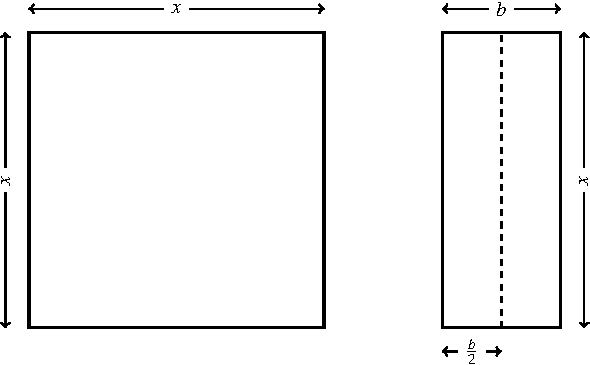
\includegraphics[scale=1]{image/09/complete-square-a1-c0.pdf}
\caption{%%
  The quadratic function $f(x) = x^2 + bx$ can be visualised as a
  square plus a rectangle.  The square has a side length of $x$, hence
  the area of the square is $x^2$.  The rectangle has a width of $b$
  and a height of $x$, so the rectangle has an area of $bx$.  Thus
  $f(x)$ can be interpreted as the area of a square plus the area of a
  rectangle.
}
\label{fig:special_complete_square_square_plus_rectangle}
\end{figure}

\end{document}
